\documentclass[12pt]{article}
\usepackage{url, graphicx}
\usepackage{geometry}
\usepackage{amsmath}
\usepackage{fancyhdr}
\pagestyle{fancy}

\title{\huge Lecture 3: The Master Theorem; The Recursive Tree Method}
\author{}
\date{}
\pagestyle{fancy}
\fancyhf{}
\lhead{COMP 251 Winter 2018}
\rhead{Lecture 3}
\lfoot{$12^{th}$ Jan, 2018}
\rfoot{\copyright{}Yutong Yan}
\cfoot{\thepage}

\begin{document}
\maketitle
\section{Quick Review}
\renewcommand{\labelitemii}{$\circ$}
\renewcommand{\labelitemiii}{$\cdot$}
\renewcommand{\labelitemiii}{$\rightarrow$}
\begin{itemize}
\item Recall, a divide-and-conquer algorithm recursively breaks up a problem of size n in smaller sub-problems such that:
	\begin{itemize}
	\item There are exactly a sub-problems.
	\item Each sub-problem has size at most {\large $\frac{1}{b}$ $\cdot$ n}
	\item Once solved, the solutions to the sub-problems can be \underline{combined} to produce 	a solution to the original problem in time $O$($n^d$)
	\end{itemize}
\item So the run-time of a divide and conquer algorithm satisfies the recurrence:

\hspace*{\fill}{\large $T$(n) = a $\cdot$ $T$($\frac{n}{b}$) + $O$($n^d$)} \hspace*{\fill} 

\item Examples: MergeSort and Binary Search
\end{itemize}


\section{The Master Theorem}
\renewcommand{\labelitemii}{$\circ$}
\renewcommand{\labelitemiii}{$\cdot$}
\renewcommand{\labelitemiii}{$\rightarrow$}
\begin{itemize}
\item \textbf{The Master Theorem}: If {\large $T$(n) = a $\cdot$ $T$($\frac{n}{b}$) + $O$($n^d$) }for constants    \\
a $>$ 0, b $>$ 1, and d $\geq$ 0 then:
\begin{center}
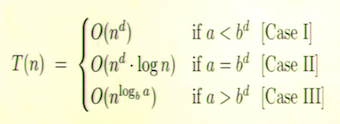
\includegraphics{lecture3a}
\end{center}
\item Sanity Check: What does this give for MergeSort and Binary Search?
\begin{center}
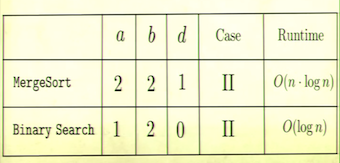
\includegraphics{lecture3b}
\end{center}
\end{itemize}
\noindent \\
\noindent \\
\noindent \\
\noindent \\
\noindent \\
\noindent \\
\noindent \\
\noindent \\
\noindent \\
\noindent \\
\noindent \\
\noindent \\
\noindent \\
\section{Proof of The Master Theorem}
\renewcommand{\labelitemii}{$\circ$}
\renewcommand{\labelitemiii}{$\cdot$}
\renewcommand{\labelitemiii}{$\rightarrow$}
\begin{itemize}
\item Fact One:
\begin{center}
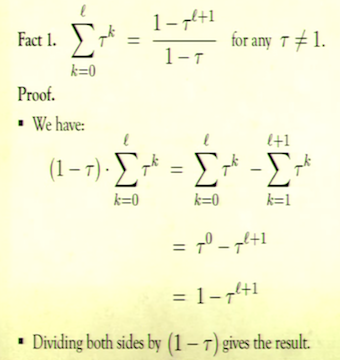
\includegraphics{lecture3c}
\end{center}
\item Fact Two:
\begin{center}
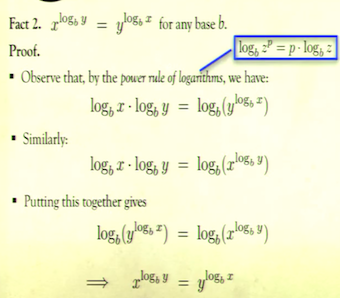
\includegraphics{lecture3d}
\end{center}

\item Proof of the Master Theorem
\begin{center}
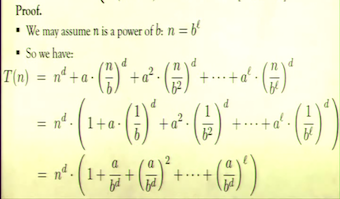
\includegraphics{lecture3e}
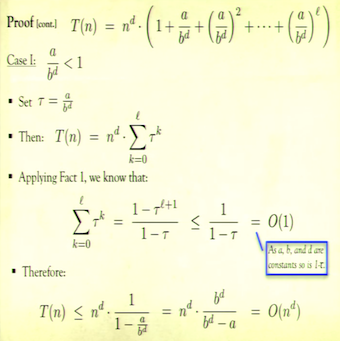
\includegraphics{lecture3f}
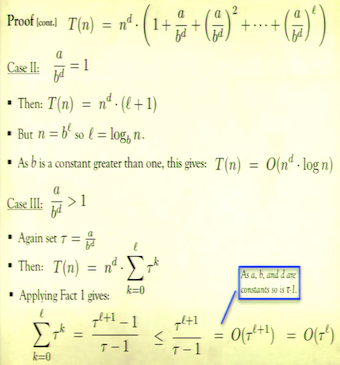
\includegraphics{lecture3g}
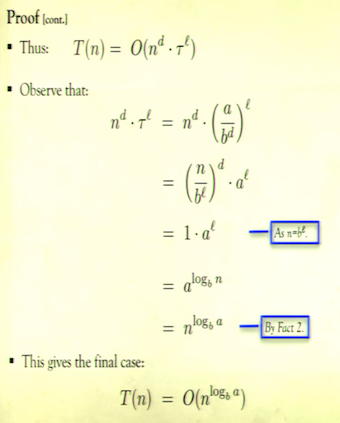
\includegraphics{lecture3h}
\end{center}
\item Specifically, what matters is \textbf{not} the statement of the Master Theorem but the \textbf{ideas} underlying its proof.
	\begin{itemize}
	\item First, if we understand the proof then we can easily reconstruct the theorem.
	\item Second, if we understand the proof then we can easily apply the method to a much 			broader class of problems. For example:
			\begin{itemize}
			\item The sub-problems have different sizes.
			\begin{center}
			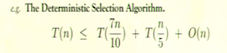
\includegraphics{lecture3i}
			\end{center}
			\item The combination function is not of the form $f$(n) = $n^d$.
			\begin{center}
			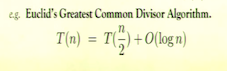
\includegraphics{lecture3j}
			\end{center}
			\item The parameters a, b, and d are \underline{not} constants.
			\begin{center}
			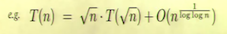
\includegraphics{lecture3k}
			\end{center}
			\end{itemize}
	\end{itemize}
\end{itemize}


\section{The Recursion Tree Method}
\begin{itemize}
\item The Master Theorem is a special case the the \textbf{recursion tree method}.
\item Specifically, we model the \textit{divide and conquer} recursive formula by a tree:

\hspace*{\fill}{\large $T$(n) = a $\cdot$ $T$($\frac{n}{b}$) + $O$($n^d$)} \hspace*{\fill} 

	\begin{itemize}
	\item The \textbf{root} node of the trees has a label n.
	\item The root has a children each with label {\large $\frac{n}{b}$}.
	\begin{center}
	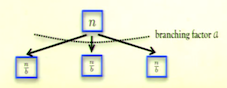
\includegraphics{lecture3l}
	\end{center}
	\end{itemize}
\item This pattern then repeats at the children, then grandchildren, etc.
\begin{center}
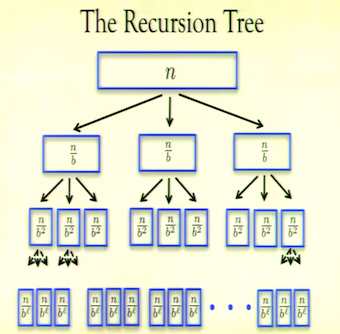
\includegraphics{lecture3m}
\end{center}
\item This process stops at the \textbf{leaves} (base cases) which have label $\frac{n}{b^{l}}$ = 1. (As n = $b^l$)
\begin{center}
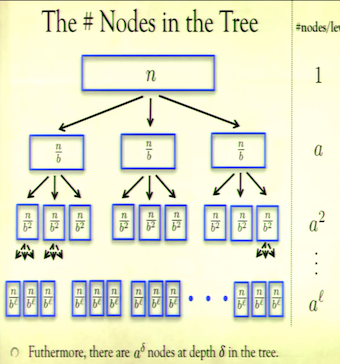
\includegraphics{lecture3n}
\end{center}
\item How much time do we spend at each level?
\begin{center}
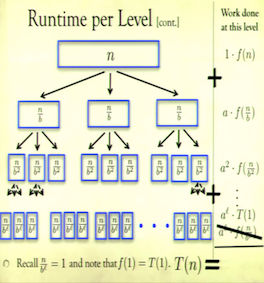
\includegraphics{lecture3o}
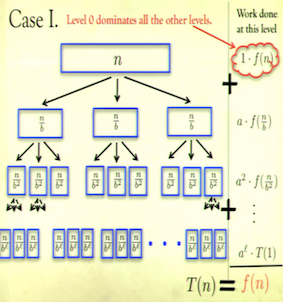
\includegraphics{lecture3p}
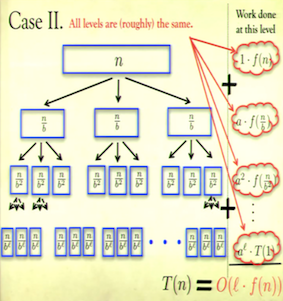
\includegraphics{lecture3q}
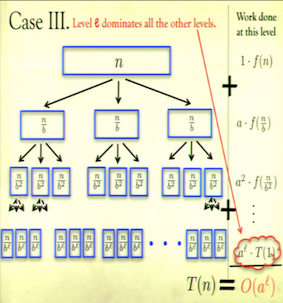
\includegraphics{lecture3r}
\end{center}
\item This gives us the proof of the Master Theorem:
\begin{center}
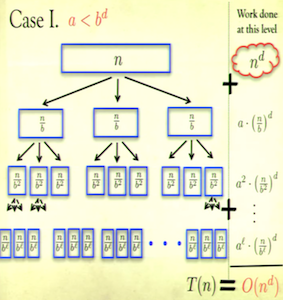
\includegraphics{lecture3s}
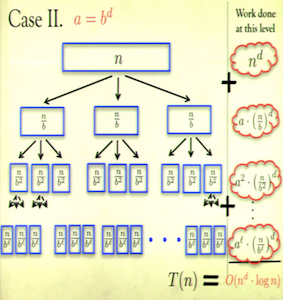
\includegraphics{lecture3t}
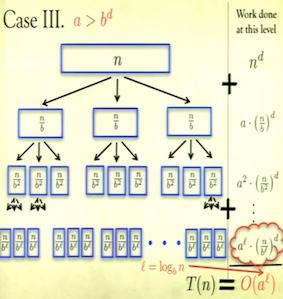
\includegraphics{lecture3u}
\end{center}

\end{itemize}















\end{document}